%\documentclass[preprints,article,accept,moreauthors,pdftex,10pt,a4paper]{Definitions/mdpi} 
\documentclass[arts,article,accept,moreauthors,pdftex,10pt,a4paper]{Definitions/mdpi} 

%=================================================================
\firstpage{1} 
\makeatletter 
\setcounter{page}{\@firstpage} 
\makeatother
\pubvolume{7}
\issuenum{1}
\articlenumber{1}
\pubyear{2018}
\copyrightyear{2018}
%\externaleditor{Academic Editor: name}
\history{Received: 30 June 2018 ; Accepted: 27 August 2018; Published: date}

%------------------------------------------------------------------
% The following line should be uncommented if the LaTeX file is uploaded to arXiv.org
%\pdfoutput=1

\updates{yes} % If there is an update available, un-comment this line

%=================================================================
% Add packages and commands here. The following packages are loaded in our class file: fontenc, calc, indentfirst, fancyhdr, graphicx, lastpage, ifthen, lineno, float, amsmath, setspace, enumitem, mathpazo, booktabs, titlesec, etoolbox, amsthm, hyphenat, natbib, hyperref, footmisc, geometry, caption, url, mdframed, tabto, soul, multirow, microtype, tikz

\usepackage[utf8]{inputenc}
\setitemize{parsep=6pt,itemsep=0pt,leftmargin=*,labelsep=5.5mm}
\setenumerate{parsep=6pt,itemsep=0pt,leftmargin=*,labelsep=5.5mm}
\setlist[description]{itemsep=0mm}   

% Bibliography
%\usepackage[
%  backend=biber,
%  style=authoryear-icomp,
%  url=true
%]{biblatex}
%\addbibresource{references.bib}

%\usepackage[]{hyperref}
%\hypersetup{
%  colorlinks=true,
%}

% Outcome tag colors and symbols:
\definecolor{enables}{HTML}{00AADD}
\definecolor{threatens}{HTML}{DDAA00}
\definecolor{advances}{HTML}{0033AA}
\definecolor{hinders}{HTML}{991100}
\newcommand{\badsym}{$\ast$}
\newcommand{\goodsym}{$\circ$}
\newcommand{\none}{{\sffamily <none>}}

% Colored outcome tags:
\newcommand{\ncemph}[1]{\textbf{\sffamily #1}}
\newcommand{\enables}{\ncemph{\color{enables}\goodsym{}\,enables}}
\newcommand{\advances}{\ncemph{\color{advances}\goodsym{}\,advances}}
\newcommand{\threatens}{\ncemph{\color{threatens}\badsym{}\,threatens}}
\newcommand{\hinders}{\ncemph{\color{hinders}\badsym{}\,hinders}}

\newcommand{\enablez}{\ncemph{\color{enables}\goodsym{}\,enable}}
\newcommand{\advancez}{\ncemph{\color{advances}\goodsym{}\,advance}}
\newcommand{\threatenz}{\ncemph{\color{threatens}\badsym{}\,threaten}}
\newcommand{\hinderz}{\ncemph{\color{hinders}\badsym{}\,hinder}}

% Non-colored tags:
% NOTE: Comment these in to remove coloring and bold face from the
% advances/hinders/enables/threatens labels.

%\renewcommand{\ncemph}[1]{{\sffamily #1}}
%\renewcommand{\enables}{\ncemph{\goodsym{}\,enables}}
%\renewcommand{\advances}{\ncemph{\goodsym{}\,advances}}
%\renewcommand{\threatens}{\ncemph{\badsym{}\,threatens}}
%\renewcommand{\hinders}{\ncemph{\badsym{}\,hinders}}
%
%\renewcommand{\enablez}{\ncemph{\goodsym{}\,enable}}
%\renewcommand{\advancez}{\ncemph{\goodsym{}\,advance}}
%\renewcommand{\threatenz}{\ncemph{\badsym{}\,threaten}}
%\renewcommand{\hinderz}{\ncemph{\badsym{}\,hinder}}

%=================================================================
% Full title of the paper (Capitalized)
\Title{Choice Poetics by Example}

% Author Orchid ID: enter ID or remove command
\newcommand{\orcidauthorA}{0000-0001-7821-1973} % Use \orcidA{} below
\newcommand{\orcidauthorB}{0000-0003-3874-1720}
\newcommand{\orcidauthorC}{0000-0002-1897-6293}
\newcommand{\orcidauthorD}{0000-0003-1964-7624}

% Authors, for the paper (add full first names)
\Author{Peter Mawhorter $^{1,}$* \orcidA{}, Carmen Zegura $^{2}$, Alex Gray $^{3}$, Arnav Jhala $^{3}$ \orcidB{}, Michael Mateas $^{4}$ \orcidC{} and Noah Wardrip-Fruin $^{4}$ \orcidD{}}
% Affiliations have been double-checked and verified with my co-authors

% Authors, for metadata in PDF
\AuthorNames{Peter Mawhorter, Carmen Zegura, Alex Gray, Arnav Jhala, Michael Mateas and Noah Wardrip-Fruin}

% Affiliations / Addresses (Add [1] after \address if there is only one affiliation.)
\address{%
  $^{1}$ \quad Computer Science \& Artificial Intelligence Laboratory, Massachusetts Institute of Technology, Cambridge, MA 02139, USA\\
$^{2}$ \quad Computer Science Department, Brown University, Providence, RI 02912, USA; carmen\_zegura@brown.edu\\
$^{3}$ \quad Computer Science Department, North Carolina State University, Raleigh, NC 27695, USA; magray2@ncsu.edu (A.G.); ahjhala@ncsu.edu (A.J.)\\
$^{4}$ \quad Computational Media Department, University of California Santa Cruz, Santa Cruz, CA 95064, USA; michaelm@soe.ucsc.edu (M.M.); nwf@soe.ucsc.edu (N.W.-F.)}
% I've double-checked these and added departments. Thanks for looking up the addresses!


% Contact information of the corresponding author
\corres{Correspondence: pmawhorter@gmail.com}

\abstract{%
Choice poetics is a formalist framework that seeks to concretely describe the impacts choices have on player experiences within narrative games.
%
Developed in part to support algorithmic generation of narrative choices, the theory includes a detailed analytical framework for understanding the impressions choice structures make by analyzing the relationships among options, outcomes, and player goals.
%
The theory also emphasizes the need to account for players' various modes of engagement, which vary both during play and between players.
%
In this work, we illustrate the non-computational application of choice poetics to the analysis of two different games to further develop the theory and make it more accessible to others.
%
We focus first on using choice poetics to examine the central repeated choice in ``\emph{Undertale},'' and show how it can be used to contrast two different player types that will approach a choice differently.
%
Finally, we give an example of fine-grained analysis using a choice from the game ``\emph{Papers, Please},'' which breaks down options and their outcomes to illustrate exactly how the choice pushes players towards complicity via the introduction of uncertainty.
%
Through all of these examples, we hope to show the usefulness of choice poetics as a framework for understanding narrative choices, and to demonstrate concretely how one could productively apply it to choices ``in the wild.''}  
% REPLY: I've removed all use of italics in the body except for use with titles. For the abstract, which is often copied without formatting applied, I've retained the use of double-quotes in addition to italics to indicate the titles of games.

\keyword{choice poetics; poetics; narrative games; choices; player goals; roleplay; complicity}

\begin{document}

\maketitle

\section{Introduction}

Originally developed in some of our prior work \citep{mawhorter2016artificial}; \citeauthor{mawhorter2014towards} (\citeyear{mawhorter2014towards}, \citeyear{mawhorter2015generating}, \citeyear{mawhorter2015intentionally}), choice poetics is a formalist framework for understanding the impact of narrative choices on the player experience via their options, their outcomes, and how those relate to player goals.
%
Choice poetics was developed in order to be deployed in a generative system that produces narrative choices, as~described in \citep{mawhorter2015generating,mawhorter2016artificial}.
%
However, the theory also supports human analysis, and~the goal of this paper is to provide examples of that.
%
We hope that these examples not only demonstrate the use of the framework, but also meaningfully contribute to existing discussions of the choices that we analyze.


\label{sec:analysis_steps}
The formal process of choice poetic analysis, having been designed with operationalization in mind, is quite detailed, but it can be summarized in four steps (concrete examples of these steps are provided below):
\begin{enumerate}
  \item \textbf{Goal Analysis}: Consider the player's mode(s) of engagement (e.g., role play, power play, etc.), and observe or assume the set of goals that influences their decisions. For a specific analysis, defining one or more player models (as prioritized set(s) of goals) is often sufficient. % Is the bold necessary? We do not encourage to use bold in the main text except titles. (SEE REPLY BELOW)
  \item \textbf{Likelihood Analysis}: Review the options offered at the choice being analyzed, and note the full range of outcomes that those options might suggest to the player, as well as the outcomes they actually produce. In addition, note how likely each suggested outcome seems to be.
  \item \textbf{Prospective Analysis}: Describe the impact of each suggested outcome on each player goal. This~gives an overall impression of how the choice will appear to the player as they encounter it, known as their prospective impression. Option/outcome patterns are recognizable at this point.
  \item \textbf{Retrospective Analysis}: Review the actual outcomes of each option, and describe their impacts on each player goal. This produces a picture of the retrospective impression that the choice will leave on the player once they observe an outcome. Pay close attention to any differences between suggested and actual outcomes. Again, specific patterns may be identifiable at this stage.
\end{enumerate}
% REPLY: The use of bold above for the four steps is the most economical way to make sure that each step title stands out, as they are key jargon for understanding the rest of the paper. I've included an alternate version that uses spacing instead of bold font to do the same job, but it's not an improvement in my opinion. Feel free to uncomment the version below if you really can't stand the bold (I've done a cursory check to make sure it doesn't screw up the rest of the layout significantly). The use of bold with the good/bad keywords is addressed along with the use of color below
%\begin{enumerate}
%  \item \hspace*{-1em} Goal Analysis \\
%    Consider the player's mode(s) of engagement (e.g., role play, power play, etc.), and observe or assume the set of goals that influences their decisions. For a specific analysis, defining one or more player models (as prioritized set(s) of goals) is often sufficient. 
%  \item \hspace*{-1em} Likelihood Analysis \\
%    Review the options offered at the choice being analyzed, and note the full range of outcomes that those options might suggest to the player, as well as the outcomes they actually produce. In addition, note how likely each suggested outcome seems to be.
%  \item \hspace*{-1em} Prospective Analysis \\
%    Describe the impact of each suggested outcome on each player goal. This~gives an overall impression of how the choice will appear to the player as they encounter it, known as their prospective impression. Option/outcome patterns are recognizable at this point.
%  \item \hspace*{-1em} Retrospective Analysis \\
%    Review the actual outcomes of each option, and describe their impacts on each player goal. This produces a picture of the retrospective impression that the choice will leave on the player once they observe an outcome. Pay close attention to any differences between suggested and actual outcomes. Again, specific patterns may be identifiable at this stage.
%\end{enumerate}
These four steps produce tables of prospective and retrospective impression labels for each option, which can usually be used to answer specific questions about a choice (e.g., ``Which option will this type of player favor?'' or ``Will the player feel this is a difficult choice?'').
%
In some cases, producing multiple contrasting analyses using different starting assumptions (such as about player goals or outcome likelihoods) can be used to answer design questions (e.g., ``Will this choice tend to separate players according to player types?'' or ``Should the likelihood of this outcome be important for how players will perceive this choice?'').

\label{sec:prospective_labels}

For prospective analysis, the valence and likelihood of outcomes can be summarized using concise labels.
%
For each option $\times$ goal, labels can be assigned depending on whether that option has likely/unlikely outcomes that advance/hinder that goal.
%
For likely outcomes, we assign the labels \advances{} and \hinders{}, and for unlikely/unknown outcomes, we use the labels \enables{} and \threatens{}.
% We do not encourage to use colorful words in papers, please change them into black color. Please also modify the tables below. 
% REPLY: The use of color here is designed specifically to increase the readability of the tables below, where in particular the two positive and two negative labels have been given colors with similar hues and the two lesser and two greater labels have been given colors with similar brightnesses. Along with color, bold type was used to accentuate the color contrast, and the result makes the tables much more legible than they'd be otherwise. Per your other comment about bold face, I've opted to use sans-serif font to pick out these key words instead of bold face, and I've added a symbol before each label to help distinguish the "good" and "bad" labels even in situations where color might not be present (e.g., when printed on a black-and-white printer or for someone who is color-blind). I've added versions of the macros without color above but left them commented out; feel free to uncomment them if you really don't want color to be used here.
Note that most option/goal combinations will receive more than one label, e.g., an advantageous but not certain option could both \threatenz{} and \advancez{} a goal. %NOTE: Should \threatenz{} and \advancez{} be changed to \threatens{} and \advances{}? REPLY: No, these versions produce "threaten" and "advance" instead of "threatens" and "advances" for verb agreement within the text although the formal labels use singular verb agreement endings.
% 
%
The assignment of prospective labels allows us to analyze the choice by comparing it to known choice structures, or just by observing patterns among the labels.


We start with an example of contrasting modes of engagement by looking at \emph{Undertale}'s central repeated choice of how to interact with wandering monsters \citep{fox2015undertale}.
%
\emph{Undertale}'s plot revolves around the player's aggression: does the player take their cue from other games and attack every ``monster'' they come across, or do they instead use the game's unusual ``Mercy'' option to avoid violence?
%
Our analysis of \emph{Undertale} examines both how that choice changes as the player learns about its outcomes, and how different goals might lead to different play styles.
%
The game reinforces both aggressive and pacifist styles but gives those players different endings to encourage dialogue within the player community.


After exploring the importance of modes of engagement, we shift focus by deconstructing a repeated choice from \emph{Papers, Please}: whether  to approve the entry permit of someone who claims to be a refugee \citep{pope2013papers}.
%
\emph{Papers, Please} uses a carefully crafted choice structure to illustrate to the player how autocratic regimes instil complicity in their citizens by manipulating uncertainty.
%
A detailed analysis of the options and outcomes involved reveals exactly how this choice structure operates, and how it would take a different form without the element of uncertainty.
%
Choice poetics is useful here because it can show explicitly how important uncertainty is to the effect achieved by \emph{Papers, Please}, illustrating not just that the game \emph{does} encourage complicity, but the subtle psychological mechanism it uses to do so.


By providing examples of the application of choice poetics ``by hand'' as opposed to by computer, we hope to inspire others to use and eventually help refine this theory.
%
Ideally, the formal structure of choice poetics can provide language to discuss choice structures precisely, and~the exhaustive analysis of goals, options, and outcomes can help analysts uncover quirks and details not readily apparent from a more gestalt perspective.
%
Although we do not believe in formalism as an ultimate goal of literary (or interactive) analysis, we do hope that this framework can become one useful tool among many for both designers and critics to better understand the impacts of narrative choices on their audiences.

\section{Related Work}

\textls[-5]{This work builds on our previous work on the theory of choice poetics.
%
In particular, our paper ``Towards a Theory of Choice Poetics'' \citep{mawhorter2014towards} provides a concise summary of the aims of the theory and the phenomena that it attempts to explain, and Peter Mawhorter's dissertation \citep{mawhorter2016artificial} contains a chapter that provides a more detailed examination of the theory, including a walkthrough of the \emph{Papers, Please} example that we also present here.
%
It is worth acknowledging the lines of inquiry that choice poetics is in dialogue with, including formalist narratology from \mbox{\cite{aristotle1917poetics}} to \cite{barthes1975introduction}, the psychology of narrative \cite{tversky1981framing}; \mbox{\cite{green2000role}}; \cite{mar2008function}; \cite{zunshine2006why}, the psychology of decision-making \cite{mellers1997decision,schwartz2002maximizing}, and of course other modern theories of interactive narrative \citep{aarseth1997cybertext,murray1997hamlet,ryan1991possible,tosca2000pragmatics,mateas2001preliminary,frasca2003ludologists,lindley2005story}.
%
The~specific ideas about modes of engagement and player motivations used here are based largely on the work of   \cite{yee2006motivations}, along with other work summarized in \citep{hamari2014player}, although choice poetics can also incorporate non-standard modes of engagement such as critical play \citep{flanagan2009critical} (see Chapter 3 of \citep{mawhorter2016artificial} for a more detailed explanation of these links).
%
Other relevant studies provide insight into how engagement can be driven by multiple desires \citep{lindley2005story}, can be affected by choices and their consequences \citep{mallon2005stand}, and can change over time \citep{lange2014youre}.
%
The development of choice poetics was also informed by non-academic writing on choice design, such as design advice for authors of online interactive narratives \citep{choiceofgames2010rules} or tabletop roleplaying game masters \citep{laws2001robin}.
%
Finally, concurrent experimental work (including some of our own) around choices and outcomes in games has provided useful empirical data about choices and their consequences \citep{fendt2012achieving,cardonarivera2014foreseeing,mawhorter2015generating,iten2018choosing}.}


\subsection{Moral Choices}

Our first analysis engages with the popular 2015 indie roleplaying game \emph{Undertale} and how players with similar goals but different priorities can be steered towards different decisions.
%
Existing scholarly literature on \emph{Undertale} has examined its portrayal of morality and ethics through its primary choice of ``kill'' or ``spare'' \citep{muller2017undertale}, the ways the game solidifies the significance of its choices through various mechanics \citep{day2017agency}, and how its musical score changes from tonal and pleasant to atonal and eerie depending on the player's approach \citep{perez2017undertale}.
%
Notably, \emph{Undertale} goes so far as to remember a player's decisions even after they ostensibly reset the game, encouraging the idea that its choices are meaningful \citep{hughes2015undertale}.
%
Although \emph{Undertale}'s designer Toby Fox has been reticent about his intentions regarding the game's moral choices, he is clearly interested in aspects of game design beyond traditional roleplaying game mechanics (quoted in \cite{feeld2015interview}):

\begin{quote}
  \itshape
The addictive quality of ``numbers increasing'' is what drives a lot of games. But some of the most important things in life can't be accurately represented by numbers.
\end{quote}


As described by Müller, Undertale's various endings have encouraged the player community to discuss attitudes towards violence both in games and in real life (\cite{muller2017undertale}, Section 2.2.1).
%
The~usefulness of choice poetics in this context is that is provides a concrete way of describing which aspects of Undertale's central kill/spare choice are mobilized to achieve this result, and by contrasting two different possible player perspectives, it illustrates how different players might naturally be encouraged to pursue different play styles and therefore observe different content, providing fodder for online discussion.
%
Of course, a formalist analysis is not the only way to reach that conclusion, but it is a mechanical and reproducible way to do so, potentially making it accessible to novice critics (and as in our prior work, to automated systems).


Broader research on moral choices in games includes examinations of their implementation and studies of how players respond to them \citep{svelch2010good,weaver2012mirrored,consalvo2016playing}.
%
Of course, research on the psychological effects of games, especially violent games, is quite popular, but has come to largely mixed conclusions \citep{ferguson2008school,ellithorpe2015moral}.
%
In fact, there is also interest in using video games to encourage better moral decision making \citep{kastarov2017training}.


\subsection{Coercion and Complicity}

In our second analysis, we  discuss complicity in \emph{Papers, Please}, and use a detailed breakdown of a single choice to illustrate how this moral issue is raised within the game.
%
A version of this analysis appears in \citep{mawhorter2016artificial}, but a more thorough analysis of the game and its themes has also been undertaken by 
Paul Formosa, Malcolm Ryan, and Dan Staines (\cite{formosa2016papers}; for~a critical perspective, see also \cite{alexander2013designing}, which Formosa et al. cite themselves).
%
Formosa, Ryan, and Staines' excellent analysis of the game and its moral dimension largely agrees with our conclusion that the game uses ambiguity as a mechanism to encourage complicity, and in fact they even quote personal correspondence with Lucas Pope, the game's designer, to the same effect: ``On some level I want players to reach a point of self-realization---about how good people can be turned into uncaring cogs'' (Pope quoted in \cite{formosa2016papers}).
%
We find these congruences encouraging, because they show that choice poetics can produce conclusions that are not only echoed by other analyses but which also seem to have been intended by the designer themselves.
%
Of course, if existing analyses have reached these conclusions already, why use choice poetics at all?
%
In this case, choice poetics provides a more detailed accounting of the importance of ambiguity in terms of the choices faced by the player, and is able to explain exactly why removing ambiguity would change a (hypothetical) player's perspective on the game.
%
Such detailed accounting of the impact of outcomes could be useful for designers interested in tweaking their choices to best support desired narrative or persuasive goals, and in fact, at least for machine-designed choices, this has shown to be somewhat effective (see \cite{mawhorter2015intentionally}).
% REPLY: I edited wording in this paragraph and the paragraph below to pull the two orphaned lines above the figure on the next page up onto this page.


Other scholarly work dealing with complicity in games is also relevant here.
%
Toby Smethurst and Stef Craps  discussed the appearance of trauma in games, including a section on complicity \citep{smethurst2015playing}.
%
In a similar vein, Holger Pötzsch  discussed complicity in games, again in the context of more scripted narrative settings \citep{potzsch2017selective}.
%
Both of these analyses include \emph{Spec Ops: The Line} \citep{yager2012spec} as an example of a game that deals with complicity, but which does so in a completely different manner to \emph{Papers, Please}, using a scripted narrative and being much more direct and extreme about the moral decisions being made (see also \cite{murray2016race} on the game's failure to grapple with issues of racism and sexism even as it does address toxic masculinity).


\section{Reinforcing Disparate Choices in \emph{Undertale}}

\emph{Undertale} is an independently developed roleplaying game \citep{fox2015undertale} about a kid trying to get back home.
%
The game appears at first to be a normal roleplaying game with some interesting mechanics, but the facade of standard RPG (role-playing game) mechanics hides a deeper morality-based storyline which challenges gamers to think more deeply about the random ``monsters'' they are fighting. %NOTE: Please define abbreviations here and every abbreviations when they are first appear,  if appropriate.
%
Players face different challenges and receive different endings depending on whether they play the game passively or aggressively.
%
These paths allow for the game to be a straightforward example of what happens when players with different play styles are forced to make the same choice.


Figure \ref{fig:UT_froggit} shows the very first random encounter of the game, and illustrates the repeated central choice of whether to fight, flee, or ``spare'' each opponent (``Flee'' and ``Spare'' are the options in the ``Mercy'' menu).
%
With the exception of certain bosses, all ``enemies'' in the game must be dealt with in one of these three ways, where killing them awards gold and experience points, fleeing gives no reward, and sparing them awards just gold, which is only possible after taking a specific sequence of actions that pacify the opponent which the player must learn for each type of ``monster.''
%
To understand how this repeated choice is set up to create dialogue within player communities, we can break it down using a formal analysis.



To simplify the analysis, we ignore concerns about player skill, which would provide an extra motive to select the ``flee'' option.
%
Although contrasting approaches to this choice across players of different skill levels would also be an interesting approach, we consider here the perspective of players that have no trouble with the challenges involved in either attacking or pacifying the enemies.

% REPLY: Changed figure placement here to [t] instead of [H].
\begin{figure}[t]
  \centering
    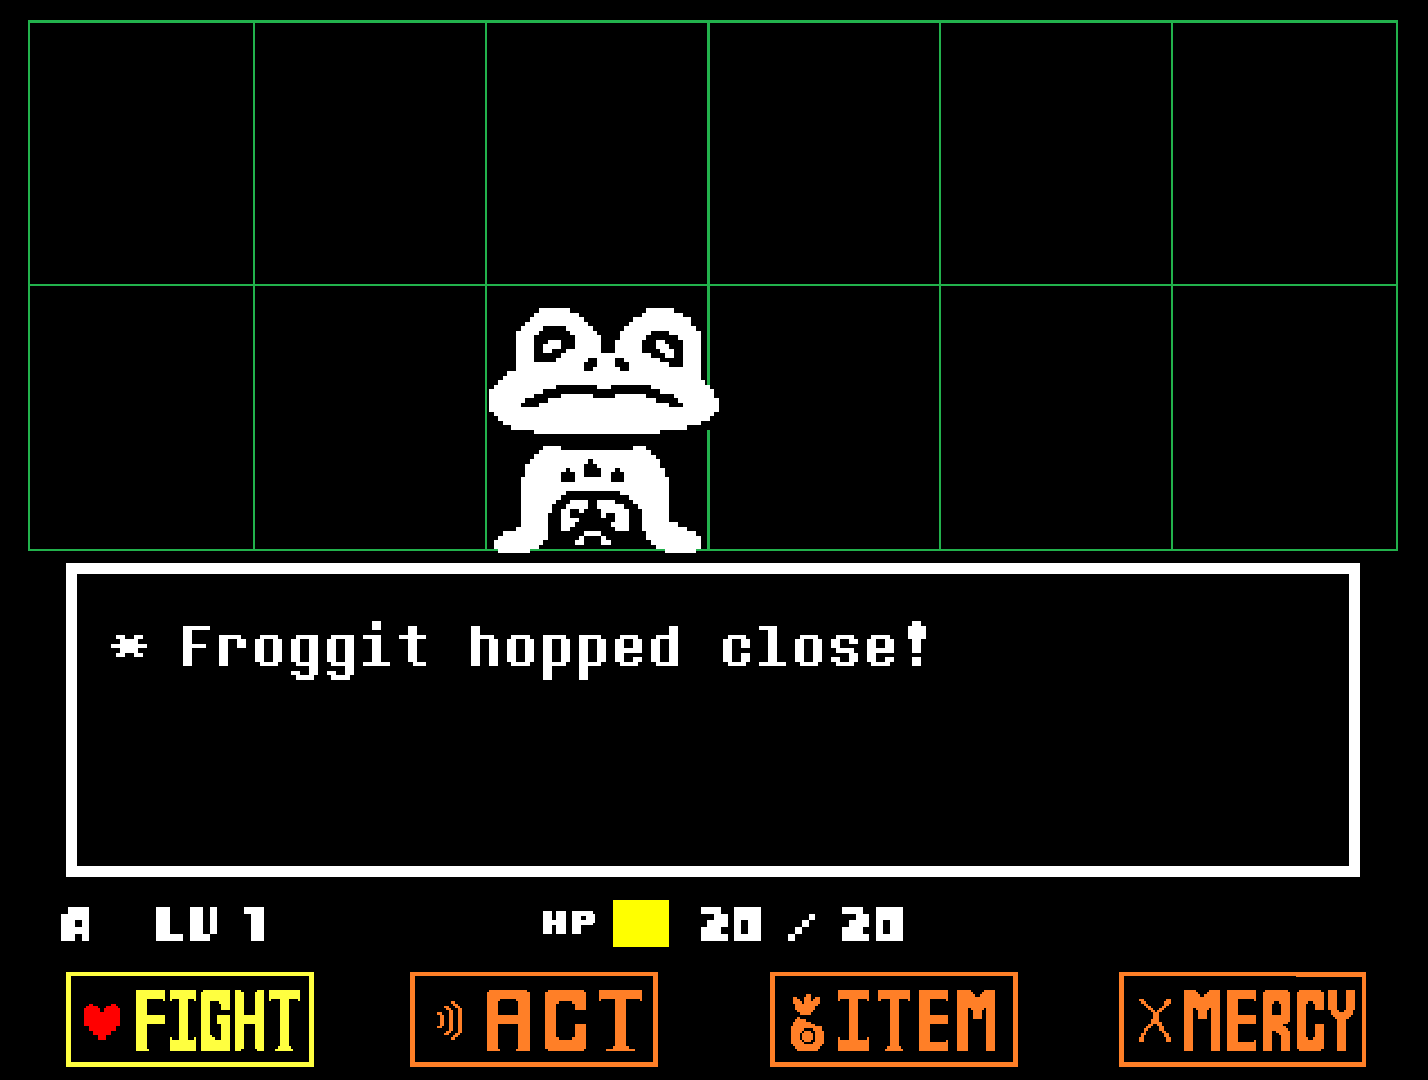
\includegraphics[width=0.8\textwidth]{fig/froggit-hopped-close-narrow.png}
    \caption{A screenshot from \emph{Undertale} showing the first random encounter of the game, in which a ``Froggit'' ``hops close'' (note that aggression is implied via the convention of a random encounter but not by the text). The options are ``fight,'' ``act,'' ``item,'' and ``mercy,'' the last of which is unconventional. Screenshot by Peter Mawhorter, licensed under Creative Commons Attribution-ShareAlike 4.0 International License (CC BY SA).}
    %We cannot publish images without permission. Please confirm you have obtained the permissions and add copyright information in each figure caption, for example “used by permission”, “photo took by author”, “in public domain” or follow copyright holders’ instructions. Please note that EVERY figure caption should have copyright information, otherwise please delete the figure. REPLY: Thanks for catching this. I've made my own screenshots and added licensing information. Some text has been changed to accommodate differences between the old and new screenshots for Papers, Please.
    
    \label{fig:UT_froggit}
\end{figure}


The remaining subsections here describe the results of each of the analysis steps outlined in Section \ref{sec:analysis_steps}, and how they differ both for two different player models and between initial and subsequent encounters with the choice.
%
Our first player model\footnote{In choice poetics, a player model is defined as a specific set of prioritized goals, which makes it more specific than a ``player type'' as used in other literature, although our player models in this analysis roughly correspond to two popular ``player types'' identified in the literature (see below).} (we call them the power player) is intended to model an experienced roleplaying game player, who is familiar with the conventions of the genre and who expects to be asked to fight their way to victory, collecting experience and gold along the way to gain power and overcome challenging bosses.
%
This power player model is grounded in the ``Achievement'' dimension of player motivation identified in \citep{hamari2014player}, which corresponds to the idea of ``power play'' as a mode of engagement \citep{mawhorter2014towards}.
%
Our~second player model (we call them the story player) attempts to approximate someone who has little experience with roleplaying games and is interested in experiencing the story of \emph{Undertale}.
%
This model is related to the dimension of player motivation that Hamari and Tuunanen identify as ``Immersion,'' and the ``avatar play'' mode of engagement from \citep{mawhorter2014towards}.

\subsection{Goal Analysis}

We use the following set of goals, with the listed power/story priorities for our respective player models (these prioritized goal sets are the player models):

\begin{itemize}
  \item Gain experience points (high/low)---The power player prioritizes experience points (XP), knowing that they may be necessary to accumulate power and beat the game. The story player understands them as a reward, but does not seek them out to the detriment of other goals.
  \item Gain gold (high/low)---Similar to XP, the power player seeks out gold while the story player welcomes it but does not prioritize it.
  \item Show mercy (none/high)---While the power player sees interactions with the monsters as instrumental and inconsequential, our hypothetical story player, swayed by the aesthetics of the game, finds them cute and feels bad being violent towards them (of course, not all story-focused players would have this outlook).
  \item Explore options (low/high)---Faced with a new game, both the power and story players are interested in figuring out what makes this game unique and what is possible within it, although for the power player this is secondary to other concerns. The ``Mercy'' menu especially, as an unconventional option, will attract interest.
  \item Behave consistently (low/low)---Both of our hypothetical players not only exhibit standard human biases towards consistent action (and justification of their past actions using future actions), but also recognize that, in most game systems, rewards are reserved for extreme behavioral profiles. This goal does not trump others, but influences ambiguous cases.
\end{itemize}
Although these exact goal sets might not be those of any actual player, they do approximate common aspects of player psychology described within existing literature (e.g., the ``Achievement'' and ``Immersion'' dimensions from \cite{hamari2014player}).
%
Any concerns about particular goals or their prioritization could always be investigated by contrasting results with yet another player model that differed from one of these in terms of the goal in question, and of course, were data on actual player goals available in some form, they could be used to define detailed player models for personalized or aggregate analysis.
%
Examples of blind playthroughs uploaded to YouTube (e.g., \cite{fuandon2015lets} for the story player model and \cite{therpgminx2015lets} for the power player model) also support the idea that these profiles might model some actual players.



\subsection{Likelihood Analysis}

\begin{table}[b]
\centering
\begin{tabular}{l l l}
  \toprule
 \multicolumn{1}{c}{\textbf{Fight}} & \multicolumn{1}{c}{\textbf{Flee}} & \multicolumn{1}{c}{\textbf{Spare}} \\
  \midrule
 (likely) Froggit dies & (likely) Froggit lives & (likely) Froggit lives \\
 (likely) XP reward & (likely) no XP & (unlikely) XP reward \\
 (likely) Gold reward & (likely) no Gold & (unlikely) Gold reward \\
 (known) New option & (known) New option & (known) New option \\
 (known) Not repeated & (known) Not repeated & (known) Not repeated \\
  \bottomrule
\end{tabular}
  \caption[\emph{Undertale} likelihood analysis]{Likelihood analysis for the player's initial encounter with the choice shown in Figure \ref{fig:UT_froggit}. The~``new option'' ``outcome'' reflects the player goal of exploring unknown options, whereas the ``repeated'' ``outcome'' reflects the player goal of behaving consistently (both are the same for all three options the first time the player encounters this choice).}
\label{tab:UT_likelihoods}
\end{table}

The next task is to decide which options suggest what outcomes, which can be tricky, as there is a wide range of possible outcomes to consider.
%
Luckily, our choice of player goals can narrow that range somewhat---for example, in this analysis, we have assumed our players are skilled enough that they will always succeed, so we ignore outcomes related to player injury or death.


Table \ref{tab:UT_likelihoods} shows likelihood analysis results for the player's first encounter with this choice (which are the same for both player models), including extradiegetic outcomes relating to exploration and consistency goals.
%
Once the player learns the actual outcomes of each choice, these likelihoods will be simplified: the player will know the true outcomes (all ``likely'' outcomes become ``known''), and~the two unlikely outcomes will be revealed (sparing rewards gold, but no XP).
%
For the extra-diegetic outcomes, players who have explored all the options will view none of them as novel, and depending on which option they picked most, they will view one as more consistent with their past behavior.



\subsection{Prospective Analysis}

Having listed a set of suggested outcomes and their likelihoods, the analysis can proceed to evaluate the prospective impressions created by this choice (as described in Section \ref{sec:prospective_labels}).
%
The results are shown in Table \ref{tab:UT_options}, which includes two versions: the block on the left shows evaluations using the initial likelihoods, while the block on the right shows the evaluations after all outcomes are known.
%
The subsequent results also use (P) and (S) to show labels that differ between the power (P) and story (S) player models (mostly, the two models just have different priorities for the different goals).
%
The~post-hoc evaluations from the right side of Table \ref{tab:UT_options} are further summarized in Table \ref{tab:UT_option_summary} which shows at a high level how many goals are advanced or hindered by each option for the two player models.

\begin{table}[t]
\centering
\begin{tabular}{c l l l l l l}
  \toprule
  & \multicolumn{3}{c}{\textbf{Initial}} & \multicolumn{3}{c}{\textbf{Subsequent}} \\
 \cmidrule{1-4} \cmidrule{5-7}
  \textbf{Goal} & \multicolumn{1}{c}{\textbf{Fight}} & \multicolumn{1}{c}{\textbf{Flee}} & \multicolumn{1}{c}{\textbf{Spare}} & \multicolumn{1}{c}{\textbf{Fight}} & \multicolumn{1}{c}{\textbf{Flee}} & \multicolumn{1}{c}{\textbf{Spare}} \\
 \cmidrule{1-4} \cmidrule{5-7}
  \multirow{2}{7em}{\centering gain-XP} & \enables{} & \hinders{} & \enables{} & \multirow{2}{4.6em}{\advances{}} & \multirow{2}{4.6em}{\hinders{}} & \multirow{2}{4.6em}{\hinders{}} \\
                                        & \advances{} & \threatens{} & \threatens{}  \\
  \cmidrule{1-4} \cmidrule{5-7}
  \multirow{2}{7em}{\centering gain-gold} & \enables{} & \hinders{} & \enables{} & \multirow{2}{4.6em}{\advances{}} & \multirow{2}{4.6em}{\hinders{}} & \multirow{2}{4.6em}{\advances{}} \\
                                          & \advances{} & \threatens{} & \threatens{}  \\
 \cmidrule{1-4}\cmidrule{5-7}
  \multirow{2}{7em}{\centering show-mercy} & \hinders{} & \enables{} & \enables{} & \multirow{2}{4.6em}{\hinders{}} & \multirow{2}{4.6em}{\advances{}} & \multirow{2}{4.6em}{\advances{}} \\
                                          & \threatens{} & \advances{} & \advances{} \\
 \cmidrule{1-4} \cmidrule{5-7}
  explore-options & \advances{} & \advances{} & \advances{} & \none{} & \none{} & \none{} \\
 \cmidrule{1-4} \cmidrule{5-7}
  \multirow{2}{7em}{\centering be-consistent} & \multirow{2}{4.6em}{\none{}} & \multirow{2}{4.6em}{\none{}} & \multirow{2}{4.6em}{\none{}} & \advances{} (P) & \multirow{2}{4.6em}{\hinders{}} & \advances{} (S) \\
  & & & & \hinders{} (S) & & \hinders{} (P) \\
  \bottomrule
\end{tabular}
  \caption[\emph{Undertale}option analysis]{Option analysis for the example choice shown in Figure \ref{fig:UT_froggit}. The results for initial and subsequent encounters are shown separately in the left and right halves of the table. All of the labels apply to both of our player models, except the be-consistent labels for the subsequent analysis, where the power (P) and story (S) player models each view either ``fight'' or ``spare'' as consistent and the other options as inconsistent (elsewhere stacked labels indicate that multiple labels apply for both models).}
\label{tab:UT_options}
\end{table}



In this case, we can see that, for both player models, the fight and spare options are more attractive than the flee option, and in fact the spare option dominates the flee option for this goal set in all cases, making it mostly irrelevant (of course, this is because we are ignoring player skill as a factor).
%
Comparing just the fight and spare options for the initial decision, we can see that the spare option is seen as a bit dubious in terms of the power-related goals, but clearly superior in terms of the mercy~goal.


Considering the power and story players, the power player is most likely to pick ``fight,'' because they ignore the show-mercy goal, so from their perspective, fight is the only option without downsides (of course considering player skill would have complicated that).
%
Meanwhile, the story player, whose highest-priority goals are to explore and show mercy, will likely pick ``spare,'' as it is best for those goals while not entirely sacrificing their low-priority goals.
%
As both of these players encounter this choice again, their explore-options goal will now favor the options they did not choose at first, and the story player may now attempt fighting, and will probably attempt fleeing, because their high-level goals of exploration and mercy are now in conflict.
%
Ultimately, the story player will find sparing most rewarding after all options have been explored.
%
In contrast, the power player, with a lower priority on exploration, may eventually try spare and/or flee out of boredom, but upon learning that those options do not award XP, they will continue to fight most enemies.


As these patterns are established, biases that promote consistency (see e.g., \citealp{brehm1956postdecision}; \mbox{\citealp{mather2000misremembrance}}; \citealp{hall2012lifting}) will be reinforced, and the power and story players will in all likelihood settle for picking fight and spare, respectively.
%
As we can see, the key factor that separates these models is their relative prioritization of the mercy goal, in conjunction with their priorities for gaining XP and gold.
%
Importantly, beyond the immediate rewards shown here, sparing monsters also leads to a number of other acknowledgements and ultimately rewards the player with the ability to befriend some of the more important characters, which is a reward well-suited to players interested in exploring a deeper story.
%
Given an audience of players with a spectrum of preferences, the game prompts different initial choices, and then encourages sticking to those choices (via consistent gold and XP rewards for fighting, and via gold and story rewards for sparing).




\subsection{Retrospective Analysis}

After making each decision, the immediate rewards are as expected.
%
However, as the game progresses, there are longer-term consequences for both systematic approaches that we consider here.
%
In particular, towards the end of the game, the story line diverges sharply, in the aggressive case throwing the player into brutal battles against several bosses, and in the passive case allowing the player to befriend some of those characters and not fight them at all (although other bosses appear)\footnote{Note that these divergences still happen even if the player does not reach one of the special endings to the game, which typically require extensive forethought and would not be reached by first-time players who do not consult a guide.}.


The long-term consequences of these individual decisions are not simply rewards or punishments, although sparing monsters leads to a happier story outcome.
%
Instead, they represent divergent worlds, which gives the player a strong sense of agency, but also causes players who take different paths and then compare notes to surprise each other.
%
By reinforcing each path separately and letting content diverge significantly, \emph{Undertale} fosters dialogue between its players, because once they learn of each others' disparate experiences, they will naturally be curious as to how those experiences were unlocked.
%
Had the game simply punished players for fighting the enemies, this would have delivered a fairly simplistic moral message, but instead, the game lets that message unfold via dialogue with other players, and as previously mentioned, uses some extra-diegetic mechanics to give its choices extra~permanence.


\subsection{Discussion}

This analysis set out with the goal of understanding how two different player models could be encouraged to routinely deal with \emph{Undertale}'s randomly-encountered ``monsters'' in different ways.
%
After understanding the prospective option impressions involved for both initial and repeated iterations of this choice, we can see that the reward structure does indeed encourage power-focused and story-focused players to take different paths, and rewards them for doing so in different ways.
%
By~deconstructing \emph{Undertale}'s repeated kill/spare choice using two generic player models, we have gotten some insight into how different players might be encouraged to explore the game differently, but of course there are other important choices and mechanics in the game that help push players down one path or the other.



As explored in Hughes' review of the game and Müller's thesis \citep{hughes2015undertale,muller2017undertale}, part of the message of \emph{Undertale} is not merely about violence itself, but about the player's willingness to callously manipulate the lives of the characters in the game.
%
The moral dichotomy that it sets up through a carefully crafted choice that will separate its audience into opposing camps serves to underline this point and get players to think deeply about it as they attempt to justify their decisions to each other (see, e.g., \cite{oh2016genocide} for an example of discussion within the player community).


The value of choice poetics here lies in explaining the mechanisms behind such narrative choices with specificity.
%
For example, in Table \ref{tab:UT_option_summary}, we can see that for our story player model, both the fight and spare options are not purely good or bad: the fight option advances some low-priority goals, while the spare option hinders one.
%
As a designer, if we wanted to tweak this choice to more strongly reinforce sparing the monsters, we could consider rewarding some XP for sparing monsters, which would cause the spare choice to dominate the fight choice for players interested in showing mercy.
%
By the same token, the choice not to do so makes the spare option more meaningful: the player actually has to make a sacrifice in order to access it, which potentially increases psychological attachment to that choice, and which might also heighten the player's sense of agency.


These kinds of detailed observations about individual outcomes are something that choice poetics enables naturally.
%
In fact, choice poetics offers a mechanism whereby approaching a choice with a specific question (e.g., ``How do power and story players approach this choice differently?'') leads to formal descriptions of that choice that can be used to answer other questions (e.g., ``How would awarding XP for sparing monsters change this choice?'').
%
In the best case, those formal descriptions or the process of their production raise further questions that highlight as-yet-unconsidered issues with the design of a choice.
%
For example, in this analysis, we noted in passing that the flee option is always dominated by one of the other options assuming the player has a certain level of skill.
%
That observation prompts the question: how do different levels of difficulty affect the player's perception of this choice, which could be answered using further comparative analysis that introduced goals related to self-preservation and player models with different skill levels (which could be modeled using outcome likelihoods for taking damage and/or dying).
%
Although there is not room here to carry out that analysis, the fact that our initial analysis suggests it is a good sign that choice poetics as a formal system can be a productive tool for these kinds of analytical projects.


\begin{table}[H]
\centering
\begin{tabular}{c c c c }
  \toprule
\multicolumn{4}{c}{\textbf{Power Player}} \\
  \midrule
  \textbf{Priority} & \textbf{Fight} & \textbf{Flee} & \textbf{Spare} \\
  \midrule
  \centering High & \advances{} $\times$ 2 & \hinders{} $\times$ 2 & \advances{} $\times$ 1, \hinders{} $\times$ 1  \\
  \midrule
  \centering Low & \advances{} $\times$ 1 & \hinders{} $\times$ 1 & \hinders{} $\times$ 1 \\
\midrule
\multicolumn{4}{c}{\textbf{Story Player}} \\
  \midrule
  \textbf{Priority} & \textbf{Fight} & \textbf{Flee} & \textbf{Spare} \\
    \midrule
  \centering High & \hinders{} $\times$ 1 & \advances{} $\times$ 1 & \advances{} $\times$ 1  \\
  \midrule
  \centering Low & \advances{} $\times$ 2, \hinders{} $\times$ 1 & \hinders{} $\times$ 3 & \advances{} $\times$ 2, \hinders{} $\times$ 1 \\
  \bottomrule
\end{tabular}
  \caption[\emph{Undertale}option summary]{Option analysis results from the right-hand (post-hoc) side of Table \ref{tab:UT_options}, grouped according to player models, options, and goal priorities. This illustrates at a high level how (after exploring each option) the power player is encouraged to fight ``monsters'' while the story player is encouraged to spare them.}
\label{tab:UT_option_summary}
\end{table}



\section{Uncertainty and Complicity in \emph{Papers, Please}}

\emph{Papers, Please} \citep{pope2013papers} gives the player the role of a border inspector in the fictional autocratic regime of Arstotzka.
%
Struggling to support their family at home, they are challenged to quickly inspect passports, visas, and eventually travel permits and vaccination records to either permit or deny entry for a stream of hopeful immigrants and travelers, earning money for each applicant correctly approved or denied.
%
A central part of the game is unresolved ambiguity, both about the identities and claims of those seeking entry and about the motives and legitimacy of the government and opposing revolutionary forces.
%
\cite{alexander2013designing} gives a nice overview of the game from a critical perspective, and \cite{formosa2016papers} provides a detailed analysis of its systemic engagement with a variety of moral issues.


Of interest to this analysis is the choice shown in Figure \ref{fig:PP_visa}, and similar choices with higher stakes which come up at several points in the game.
%
In each case, the player must decide whether to take someone at their word that, despite a missing or incorrect document, they still deserve admission.
%
This decision is complicated by the fact that the game also presents situations where applicants attempt to bribe or threaten the player, implying that not all of their claims can be taken at face value.
%
This decision about the fate of an ostensible refugee (or similar person) embodies one of the central themes of the game: how the uncertainty of information from unreliable sources can be pitted against the certain plight of one's family to turn a moral dilemma into a choice with a reluctant ``better'' option.
%
In the rest of this section, we show the results of each step of a choice poetic analysis (see Section \ref{sec:analysis_steps}) for the choice described in Figure \ref{fig:PP_visa}.


\begin{figure}[H]
  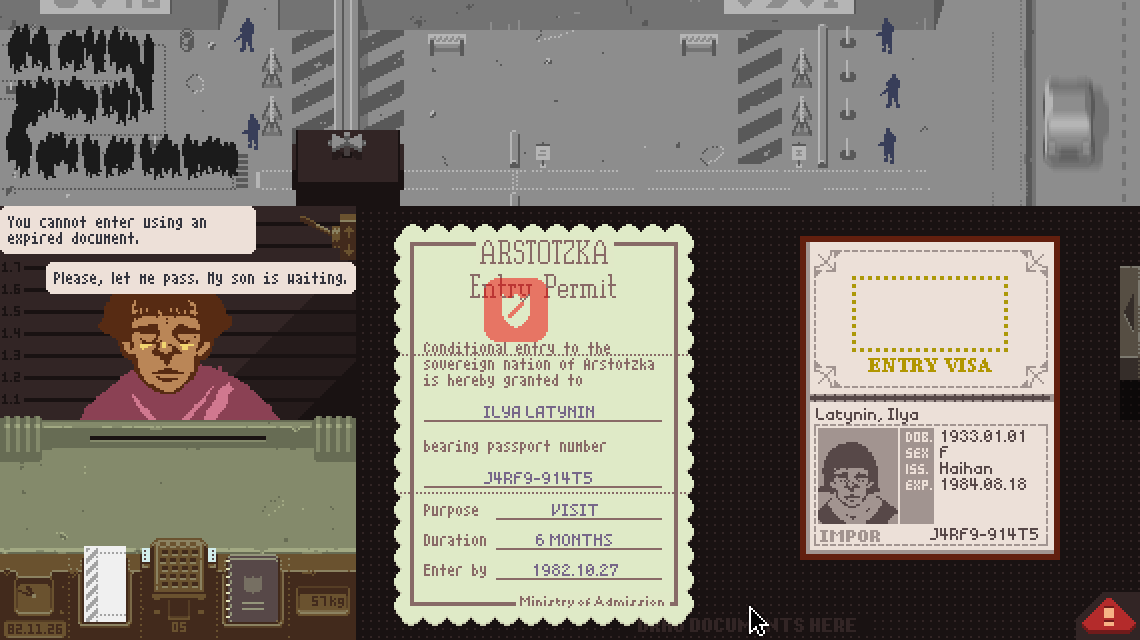
\includegraphics[width=\textwidth]{fig/please-son-waiting.png}
  \caption{A screenshot from \emph{Papers, Please} showing the interface as the player decides whether to admit a traveler. The traveler in question previously stated that she was coming to visit her son, who she has not seen in 6 years. Although her entry permit is slightly out-of-date, she is asking for leniency. At this point, the player must decide to either approve or deny her visa. Screenshot by Peter Mawhorter, licensed under CC BY SA.}
  \label{fig:PP_visa}
\end{figure}


\subsection{Goal Analysis}

For the purposes of understanding this choice, it is sufficient to use a single player model with the following prioritized goals:
\begin{itemize}
  \item (high-priority) Provide for your family---the player wants to earn credits and avoid penalties to be able to pay for food and shelter at the end of the day.
  \item (high-priority) Act ethically---as much as possible, the player wants to treat applicants ethically and avoid acting in ways that would harm them without a proportionate justification, even when this goes against the government's dictates.
  \item (medium-priority) Apprehend criminals---separate from their desire to earn credits, the player actively wants to identify applicants who might be attempting to gain entry to the country deceitfully and reject their applications.
  \item (low-priority) Admit approved travellers---all else being equal, the player seeks to treat applicants fairly and admit those that have everything in order.
\end{itemize}
If we were concerned about differences between players, we could repeat this analysis with another set of player goals and contrast the results, as we did with \emph{Undertale}.
%
Note that, especially in this case, the results of the analysis inform and justify the player model used.
%
If results differ significantly from what we know about a choice, there are two possibilities: either one or more of our assumptions (about goals, goal priorities, and/or the perception of outcomes) was wrong, in which case we can revise or extend our assumptions and re-do the analysis, or what we thought we knew was wrong, and we should be able to use our analysis to demonstrate why.
%
In this case, we think, based on other analyses and interviews with the game designer, that \emph{Papers, Please} uses ambiguity to encourage complicity, and through a formal analysis, we should be able to either back up that intuition or demonstrate why things do not actually work that way.


Because choice poetics makes its assumptions about player motivations and perceived outcome likelihoods explicit, these aspects of the analysis can be easily examined and criticized.
%
In many cases, the most efficient means of dealing with such criticism is to expand the analysis or contrast it with a proposed alternative.
%
When an analysis disagrees with other sources, the source of that disagreement is often differing assumptions about how players will perceive a choice or about how they will respond to the options offered.
%
Making those assumptions explicit thus helps ground potential disagreements, and not only allows for stating disagreements clearly (e.g., ``I don't think that most players will place a high priority on acting ethically.'') but allows for alternative assumptions to be tested using an identical analytical process.


When an analysis agrees with other sources in its conclusions, the burden is on the critic to argue why a specific choice of goal priorities or outcome likelihoods is unrealistic, and demonstrate how that affects the overall argument put forward.
%
Ideally, of course, such questions might also be settled by gathering real data about player perceptions of goals and outcomes, and choice poetics provides a framework for doing so (see \cite{mawhorter2015intentionally}).



\subsection{Likelihood Analysis}

Table \ref{tab:PP_likelihoods} shows a breakdown of outcomes and their likelihoods for both possible decisions; relevant outcomes have been essentially intuited from player goals.
%
Note in particular the outcomes with unknown likelihood that represent competing possible worlds with respect to the trustworthiness of the applicant: if they are telling the truth about their plight, admitting them realizes a different outcome than if they are just making up their story to gain entrance, and the player does not have enough information to make an informed judgement either way.

\begin{table}[b]
\centering
\begin{tabular}{l l}
  \toprule
  \multicolumn{1}{c}{\textbf{Approve}} & \multicolumn{1}{c}{\textbf{Deny}} \\
  \midrule
  (likely) Do not earn a credit & (likely) Earn a credit \\
  (likely) Get punished & (likely) No punishment \\
  (unknown) Refugee is saved & (unknown) Refugee is condemned \\
  (unknown) Scam is rewarded & (unknown) Scam is thwarted \\
  \bottomrule
\end{tabular}
\caption[\emph{Papers, Please} likelihood analysis]{Likelihood analysis for the choice shown in Figure \ref{fig:PP_visa}.}
\label{tab:PP_likelihoods}
\end{table}


\subsection{Prospective Analysis}

The prospective analysis results are shown on the left side of Table \ref{tab:PP_options}; note that one of the goals (that of admitting approved applicants) is irrelevant here.
%
From these results, we can immediately see that, although both options threaten some goals, the deny option is clearly better with regards to the high-priority goal of feeding your family.
%
In fact, although approving the applicant might be an ethical action, that is not certain, and denying the applicant might also be in line with our player model's ethical standards if in fact they are making up their story.


While this choice does not contain any well-known outcome patterns (cf. \cite{mawhorter2014towards}), it does involve some moral concerns, pitting one's desire to help one's family against concerns about turning away a refugee.
%
The structure is clarified further if we consider the same analysis under the assumption that the applicant is telling the truth, which is shown on the right side of Table \ref{tab:PP_options}.
%
This~new analysis has the structure of a classic dilemma: Two options, each of which \hinders{} an equally important goal.
%
Compared to the left side of Table \ref{tab:PP_options}, concerns about apprehending criminals are gone, and the refugee-related outcomes, now believed to be likely, make the moral weight of the decision unambiguous.


This comparison thus illustrates exactly how \emph{Papers, Please} (and governments) can manufacture complicity: by introducing doubts about the motives of strangers while emphasizing the certainty of outcomes for loved ones, a dilemma that clearly warrants serious moral concern can be transformed into an uneven choice where multiple avenues of justification are available.
%
Note in particular that the player model's goal of apprehending criminals was not a deciding factor in this case.
%
Regardless of the existence of that goal, uncertainty about the applicant's situation still eliminates any \advances{} labels from the ``Approve'' column while leaving the ``Deny'' column \hinders{}-free.
%
The ambiguous decision is still not an easy one, as evidenced by the fact that it \threatens{} a top-priority goal (behaving ethically).
%
This leaves the player feeling uneasy about the decision, and potentially helps prompt more reflection on the decision, but ultimately our player model will still view denying the application as the better choice once uncertainty is introduced.



\begin{table}[H]
\centering
\begin{tabular}{c l l l l }
  \toprule
  & \multicolumn{2}{c}{\textbf{With Suspicion}} & \multicolumn{2}{c}{\textbf{Without Suspicion}} \\
  \midrule
  \textbf{Goal} & \multicolumn{1}{c}{\textbf{Approve}} & \multicolumn{1}{c}{\textbf{Deny}} & \multicolumn{1}{c}{\textbf{Approve}} & \multicolumn{1}{c}{\textbf{Deny}} \\
    \midrule
  \multirow{2}{9em}{\centering provide-for-family} & \threatens{} & \enables{} & \threatens{} & \enables{} \\
                                        & \hinders{} & \advances{} & \hinders{} & \advances{} \\
  \midrule
  \multirow{2}{9em}{\centering act-ethically} & \multirow{2}{6em}{\enables{}} & \multirow{2}{6em}{\threatens{}} & \enables{} & \threatens{} \\
  & & & \advances{} & \hinders{} \\
  \midrule
  apprehend-criminals & \threatens{} & \enables{} & \none{} & \none{} \\
  \midrule
  admit-approved & \none{} & \none{} & \none{} & \none{} \\
  \bottomrule
\end{tabular}
  \caption[\emph{Papers, Please} option analysis]{Option analysis for the example choice shown in Figure \ref{fig:PP_visa}. The default analysis is shown on the left (``With Suspicion''), and a revised analysis assuming that the player trusts the applicant (``Without Suspicion'') is shown on the right. See Section \ref{sec:prospective_labels} for how the labels were applied.}
\label{tab:PP_options}
\end{table}

\subsection{Retrospective Analysis}

At the end of each day in \emph{Papers, Please}, the player is paid based on the number of applicants they processed ``correctly,'' and then must decide how much money to allocate for family needs, such as food, heating, and eventually, medicine.
%
However, except in a few special cases, there is no information provided about the subsequent outcomes for the applicants who have entered the country that day.
%
In cases where information is available, it is as likely to raise more suspicions as assuage them: The player is eventually asked to participate in a plot to overthrow the Arstotzkan government, and both sides of the conflict are presented as having questionable motives.
%
The player is thus not given many chances to justify their beliefs about the truth of applicants' statements, and in some cases, is given extra reasons to doubt them.
%
Of course, such blanket beliefs about future applicants based on past applicants are simple biases, not rational conclusions, because the applicants are independent of each other, but they would help assuage the player's conscience (or potentially inflame it if the evidence contradicted the player's assumptions).
%
However, by denying even such a false sense of closure, the~game encourages the player to feel vaguely uneasy about their role.



At the same time, by emphasizing the outcomes for the player's family, the game pushes the player away from the dilemma mindset and towards an obvious justification for complicity: the player ``had'' to act in the state's interests because their family's welfare was at stake.
%
From a choice poetic perspective, this choice thus has two interesting properties: First, certain outcomes remain hidden from the player indefinitely, and second, the outcomes that are apparent are emphasized in the course of continued play.
%
The withholding of information serves the purpose of introducing and even emphasizing the uncertainty about outcomes that tilts the choice as discussed above, while the emphasis on the relatively certain outcomes gives the player an extra push towards viewing the choice not as a moral dilemma but as a situation where there is only one ``correct'' choice.

\subsection{Discussion}

As with our \emph{Undertale} analysis, the conclusions we reach are the same as those of other analysts \citep{alexander2013designing,formosa2016papers}, which is encouraging, because it validates our methodology.
%
At~the same time, the level of detail we achieve enables us to answer further questions: how exactly does ambiguity play a role in encouraging complicity in \emph{Papers, Please}, and what changes in player mindset or choice specifics might lead to a different outcome?


Having set out to understand how exactly \emph{Papers, Please} uses ambiguity to encourage complicity, we have used choice poetics to provide a detailed explanation of the mechanisms behind this effect.
%
The comparison presented in Table \ref{tab:PP_options} shows that suspicion about the motives of petitioners is key to turning a dilemma into a more murky and lopsided choice.
%
From this detailed analysis, we can also see which aspects of the player's mindset are necessary for this effect to occur: The player model's goal of apprehending criminals is surprisingly irrelevant to the deconstruction of the dilemma, because the goal of providing for one's family pushes in the same direction and is more clearly established by the context of the decision.
%
What is important instead is the player's willingness to be persuaded that some applicants do not deserve entry, and that denying them entry would be a good thing.
%
An~anarchist player who believed that denying anyone entry was immoral (or at least, that some balance of honest and dishonest applicants should always be resolved to favor the honest applicants) would resist the technique used here and face a clear dilemma between feeding their family and obeying their conscience.


\section{Conclusions}

Through our analyses of choices from \emph{Undertale} and \emph{Papers, Please}, we have demonstrated the concrete application of choice poetics to two very different choices.
%
As already mentioned, the conclusions drawn here about both games have already been reached by others, which confirms that our analytical approach leads to sound conclusions.
%
Relative to a typical close reading approach, choice poetics provides extra formal structure that encourages detailed observation and which can lead to secondary observations about the choice being analyzed.
%
In addition, where a close reading uses the author's experience to stand in for the experience of players, choice poetics forces the analyst to create explicit player models, thus reifying their assumptions about how choices will be perceived and opening them up for examination.
%
The assumptions that choice poetics makes about player goals are thus both a weakness (they might be wrong) and a strength (errors can be identified exactly, and contrasting analyses can test hypotheses about player goals).


Besides encouraging more explicit examination of choices, we also hope that a formalist framework can make analysis more accessible to novice critics, allowing them to systematically identify interesting aspects of a choice, and that it can provide precise language for describing narrative choices and their poetic effects.
%
Ideally, choice poetics should support discussions about why and how a choice achieves its poetic effect, and should enable those discussions to be more detailed and specific.


To explore modes of engagement, we gave an example of paired choice analysis with a central and recurring choice from \emph{Undertale}, showing how choice poetics can be used to contrast different play styles.
%
The benefit in this case was a detailed look at how \emph{Undertale} separates players with different priorities into different choice patterns to encourage dialogue between players who experience the game differently, including how divergence is encouraged at both initial and subsequent encounters with a repeated choice.
%
Choice poetics helps pinpoint exactly which outcomes drive that separation, and what sets of priorities are necessary for it to happen.


We then went into depth with \emph{Papers, Please}, using prospective and retrospective analysis to pin down subtle characteristics of a common choice in that game.
%
Noting how uncertainty undermined a dilemma configuration for that choice, we were able to describe in detail how that choice tilts players towards complicity with the game's fictional regime, and what other aspects of the choice design help contribute to this outcome.
%
In fact, our analysis reveals several simple changes that could have been implemented had the author wished to create a different narrative.
%
For example, revealing after-the-fact that most applicants begging for asylum were in fact refugees would be enough to permit a story where the player bravely resists their regime's authoritarian tendencies by turning the present ambiguous choice into a clear moral dilemma.
%
The utility of choice poetics here then is to identify exactly how a choice creates a certain feeling, and which elements of the choice might be changed to create a different one.


In all of the analyses presented here, we engage with choice poetics as human scholars, using only those pieces of the theory that are relevant to the specific choices at hand and glossing over details that seem evident from common sense.
%
Although choice poetics was designed with operationalization in mind, our analyses show that it can also be of use to human critics as a framework for discussion.
%
We~also expect that the framework's systematic steps will be useful when confronted with choices that are difficult to understand, and that the notion of different player models will help illuminate choices that leave different actual players feeling different things.


As we continue to develop this theory, we plan to explore further computational models and collect and analyze play traces to demonstrate the theory's utility in the domain of automated analysis, with the eventual goal of using it for on-line player modeling to enable responsive stories.
%
Additionally, we hope to remain in dialogue with critics and games scholars who seek to understand narrative choices, and hope that our framework can at least provide useful language to this community for discussing poetic choices.
%
Of course, we will also continue examining games, and may come up with more examples of how choice poetics can be productively applied to understanding how their choices fit into their narratives.

%%%%%%%%%%%%%%%%%%%%%%%%%%%%%%%%%%%%%%%%%%
\vspace{6pt} 

% Supplementary material
%\supplementary{None.}

%%%%%%%%%%%%%%%%%%%%%%%%%%%%%%%%%%%%%%%%%%
\authorcontributions{Conceptualization, all authors; Investigation, P.M., C.Z., A.G. and A.J.; Writing--Original Draft Preparation, P.M., C.Z. and A.G.; and Writing--Review and Editing, P.M. and N.W.-F.}

%%%%%%%%%%%%%%%%%%%%%%%%%%%%%%%%%%%%%%%%%%
\funding{The authors would like to acknowledge the support of National Science Foundation grant IIS-1409992, which supported some of the initial development of choice poetics.}

%%%%%%%%%%%%%%%%%%%%%%%%%%%%%%%%%%%%%%%%%%
\conflictsofinterest{The authors declare no conflict of interest.}

%%%%%%%%%%%%%%%%%%%%%%%%%%%%%%%%%%%%%%%%%%
\reftitle{References}
\begin{thebibliography}{999}

\bibitem[\protect\citeauthoryear{Aarseth}{Aarseth}{1997}]{aarseth1997cybertext}
Aarseth, Espen~J. 1997.
\newblock {\em Cybertext: Perspectives on Ergodic Literature}.
\newblock Baltimore: JHU Press.

\bibitem[\protect\citeauthoryear{Alexander}{Alexander}{2013}]{alexander2013designing}
Alexander, Leigh. 2013.
\newblock Designing the Bleak Genius of {\emph{Papers, Please}}.
\newblock Available online:
  \href{http://www.gamasutra.com/view/news/199383/Designing_the_bleak_genius_of_Papers_Please.php}{\nolinkurl{http://www.gamasutra.com/view/news/199383/Designing_the_bleak_genius_of_Papers_Please.php}}
  (accessed on 22 May 2018).

\bibitem[\protect\citeauthoryear{Aristotle}{Aristotle}{1917}]{aristotle1917poetics}
Aristotle. 1917.
\newblock {\em The Poetics of Aristotle}.
\newblock London: Macmillan.

\bibitem[\protect\citeauthoryear{Barthes and Duisit}{Barthes and
  Duisit}{1975}]{barthes1975introduction}
Barthes, Roland, and Lionel Duisit. 1975.
\newblock An introduction to the structural analysis of narrative.
\newblock {\em New Literary History\/}~{6\/}: 237--72.

\bibitem[\protect\citeauthoryear{Brehm}{Brehm}{1956}]{brehm1956postdecision}
Brehm, Jack~W. 1956.
\newblock Postdecision changes in the desirability of alternatives.
\newblock {\em The Journal of Abnormal and Social Psychology\/}~{52\/}: 384.

\bibitem[\protect\citeauthoryear{Cardona-Rivera, Robertson, Ware, Harrison,
  Roberts, and Young}{Cardona-Rivera
  et~al.}{2014}]{cardonarivera2014foreseeing}
Cardona-Rivera, Rogelio Enrique, Justus Robertson, Stephen G. Ware, Brent E. Harrison, David L. Roberts, and Robert Michael Young. 2014.
\newblock Foreseeing meaningful choices.
\newblock Paper presented at the 10th Artificial Intelligence and Interactive Digital
  Entertainment Conference, Raleigh, NC, USA, October 3--7.

\bibitem[\protect\citeauthoryear{Consalvo, Busch, and Jong}{Consalvo
  et~al.}{2016}]{consalvo2016playing}
Consalvo, Mia, Thorsten Busch, and Carolyn Jong. 2016.
\newblock Playing a better me: How players rehearse their ethos via moral
  choices.
\newblock {\em Games and Culture\/}~{11\/}: 1--20.
\newblock
 doi:10.1177/1555412016677449.

\bibitem[\protect\citeauthoryear{Day and Zhu}{Day and
  Zhu}{2017}]{day2017agency}
Day, Timothy, and Jichen Zhu. 2017.
\newblock Agency informing techniques: {Communicating} player agency in
  interactive narratives.
\newblock Paper presented at the 12th International Conference on the
  Foundations of Digital Games (FDG~'17), New York, NY, USA, August 14--17. New York: ACM, pp. 56:1--56:4.
  \newblock
  doi:10.1145/3102071.3106363.

\bibitem[\protect\citeauthoryear{Ellithorpe, Cruz, Velez, Ewoldsen, and
  Bogert}{Ellithorpe et~al.}{2015}]{ellithorpe2015moral}
Ellithorpe, Morgan E., Carlos Cruz, John A. Velez, David R. Ewoldsen, and Adam K. Bogert. 2015.
\newblock Moral license in video games: {When} being right can mean doing
  wrong.
\newblock {\em Cyberpsychology, Behavior, and Social Networking\/}~{18\/}: 203--207.
\newblock PMID 25803312.
  doi:10.1089/cyber.2014.0599.

\bibitem[\protect\citeauthoryear{Fabulich}{Fabulich}{2010}]{choiceofgames2010rules}
Fabulich, Dan. 2010.
\newblock 5 Rules for Writing Interesting Choices in Multiple Choice Games.
\newblock Available online:
  \href{http://www.choiceofgames.com/2010/03/5-rules-for-writing-interesting-choices-in-multiple-choice-games/}{\nolinkurl{http://www.choiceofgames.com/2010/03/5-rules-for-writing-interesting-choices-in-multiple-choice-games/}}
  (accessed on 22 June 2018).

\bibitem[\protect\citeauthoryear{Feeld}{Feeld}{2015}]{feeld2015interview}
Feeld, Julian. 2015. % Is this ``9'' a date or month?  It is not necessary to include date and month information here. Please check and modify. REPLY: These were months. I added them to the bibliography file for completeness but was thinking about figuring out a way to remove them via a style tweak. I've simply removed them by hand where highlighted here.
\newblock Interview: Toby Fox of Undertale.
\newblock Available online:
  \href{http://outermode.com/interview-toby-fox-undertale}{\nolinkurl{http://outermode.com/interview-toby-fox-undertale}}
  (accessed on 22 June 2018).

\bibitem[\protect\citeauthoryear{Fendt, Harrison, Ware, Cardona-Rivera, and
  Roberts}{Fendt et~al.}{2012}]{fendt2012achieving}
Fendt, Matthew~William, Brent Harrison, Stephen~G. Ware, Rogelio~E.
  Cardona-Rivera, and David~L. Roberts. 2012.
\newblock Achieving the illusion of agency.
\newblock In {\em Interactive Storytelling}. Berlin: Springer, pp. 114--25. 

\bibitem[\protect\citeauthoryear{Ferguson}{Ferguson}{2008}]{ferguson2008school}
Ferguson, Christopher~J. 2008.
\newblock The school shooting/violent video game link: {Causal} relationship or
  moral panic?
\newblock {\em Journal of Investigative Psychology and Offender
  Profiling\/}~{5\/}: 25--37.

\bibitem[\protect\citeauthoryear{Flanagan}{Flanagan}{2009}]{flanagan2009critical}
Flanagan, Mary. 2009.
\newblock {\em Critical Play: Radical Game Design}.
\newblock Cambridge: The MIT Press.

\bibitem[\protect\citeauthoryear{Formosa, Ryan, and Staines}{Formosa
  et~al.}{2016}]{formosa2016papers}
Formosa, Paul, Malcolm Ryan, and Dan Staines. 2016.
\newblock {\emph{Papers, Please}} and the systemic approach to engaging ethical
  expertise in videogames.
\newblock {\em Ethics and Information Technology\/}~{18\/}: 211--25.
\newblock
  doi:10.1007/s10676-016-9407-z.

\bibitem[\protect\citeauthoryear{Fox}{Fox}{2015}]{fox2015undertale}
Fox, Toby. 2015.
\newblock \emph{Undertale}.
\newblock Self-Published.
\newblock Various platforms.


\bibitem[\protect\citeauthoryear{Frasca}{Frasca}{2003}]{frasca2003ludologists}
Frasca, Gonzalo. 2003. 
\newblock Ludologists love stories, too: Notes from a debate that never took
  place.
\newblock In~{\em Level up Conference Proceedings}. JE Utrecht: University of Utrecht.
% Month is not necessary here, can be deleted or not? REPLY: Removed


\bibitem[\protect\citeauthoryear{fuandon}{fuandon}{2015}]{fuandon2015lets}
fuandon. 2015.% Is this ``9'' a date or month?  It is not necessary to include date and month information here. Please check and modify. REPLY: Removed
\newblock {Let's Play Undertale! [BLIND] Part 1: Hello, Mom}.
\newblock Available online:
  \href{https://www.youtube.com/watch?v=plvjJx-ERWY}{\nolinkurl{https://www.youtube.com/watch?v=plvjJx-ERWY}}
    (accessed on 16 August 2018).

\bibitem[\protect\citeauthoryear{Green and Brock}{Green and
  Brock}{2000}]{green2000role}
Green, Melanie~C., and Timothy~C. Brock. 2000.
\newblock The role of transportation in the persuasiveness of public
  narratives.
\newblock {\em Journal of Personality and Social Psychology\/}~{79\/}: 701.

\bibitem[\protect\citeauthoryear{Hall, Johansson, and Strandberg}{Hall
  et~al.}{2012}]{hall2012lifting}
Hall, Lars, Petter Johansson, and Thomas Strandberg. 2012, 09.
\newblock Lifting the veil of morality: {Choice} blindness and attitude
  reversals on a self-transforming survey.
\newblock {\em PLoS ONE\/}~{7\/}: 1--8.
\newblock
  doi:10.1371/journal.pone.0045457.

\bibitem[\protect\citeauthoryear{Hamari and Tuunanen}{Hamari and
  Tuunanen}{2014}]{hamari2014player}
Hamari, Juho, and Janne Tuunanen. 2014.
\newblock Player types: A meta-synthesis.
\newblock {\em Transactions of the Digital Games Research Association\/}~1: {29--53\/}.% Please add the page range. REPLY: Done

\bibitem[\protect\citeauthoryear{Hughes}{Hughes}{2015}]{hughes2015undertale}
Hughes, William. 2015.% Is this ``12'' a date or month?  It is not necessary to include date and month information here. Please check and modify. REPLY: Removed
\newblock Undertale dares players to make a mistake they can never take back.
\newblock Available online:
  \href{https://games.avclub.com/undertale-dares-players-to-make-a-mistake-they-can-neve-1798287299}{\nolinkurl{https://games.avclub.com/undertale-dares-players-to-make-a-mistake-they-can-neve-1798287299}}
  (accessed on 22 June 2018).


\bibitem[\protect\citeauthoryear{Iten, Steinemann, and Opwis}{Iten
  et~al.}{2018}]{iten2018choosing}
Iten, Glena~H., Sharon~T. Steinemann, and Klaus Opwis. 2018.
\newblock Choosing to help monsters: {A} mixed-method examination of meaningful
  choices in narrative-rich games and interactive narratives.
\newblock Paper presented at the 2018 ACM CHI Conference on Human Factors in Computing
  Systems, Montreal, QC, Canada, \mbox{April 21--26}.

\bibitem[\protect\citeauthoryear{Katsarov, Christen, Mauerhofer, Schmocker, and
  Tanner}{Katsarov et~al.}{2017}]{kastarov2017training}
Katsarov, Johannes, Markus Christen, Ralf Mauerhofer, David Schmocker, and
  Carmen Tanner. 2017.
\newblock Training moral sensitivity through video games: A review of suitable
  game mechanisms.
\newblock {\em Games and Culture\/}~{12\/}: 1--23.
\newblock
  doi:{\changeurlcolor{black}\href{https://doi.org/10.1177/1555412017719344}{\detokenize{10.1177/1555412017719344}}}.

\bibitem[\protect\citeauthoryear{Lange}{Lange}{2014}]{lange2014youre}
Lange, Amanda. 2014.
\newblock ``you're just gonna be nice:'' {H}ow players engage with moral choice
  systems.
\newblock {\em Journal of Games Criticism\/}~{1\/}: 1--16.

\bibitem[\protect\citeauthoryear{Laws}{Laws}{2001}]{laws2001robin}
Laws, Robin. 2001.
\newblock {\em Robin's Laws of Good Game Mastering}.
\newblock Austin: Steve Jackson Games.

\bibitem[\protect\citeauthoryear{Lindley}{Lindley}{2005}]{lindley2005story}
Lindley, Craig~A. 2005.
\newblock Story and narrative structures in computer games.
\newblock In {\em Developing Interactive Narrative Content:
  Sagas/Sagasnet Reader}. Edited by Brunhild~Bushoff. Munich: High Text Verlag.

\bibitem[\protect\citeauthoryear{Mallon and Webb}{Mallon and
  Webb}{2005}]{mallon2005stand}
Mallon, Bride, and Brian Webb. 2005.
\newblock Stand up and take your place: {I}dentifying narrative elements in
  narrative adventure and role-play games.
\newblock {\em Computers in Entertainment\/}~{3\/}: 6.

\bibitem[\protect\citeauthoryear{Mar and Oatley}{Mar and
  Oatley}{2008}]{mar2008function}
Mar, Raymond~A., and Keith Oatley. 2008.
\newblock The function of fiction is the abstraction and simulation of social
  experience.
\newblock {\em Perspectives on Psychological Science\/}~{3\/}: 173--92.

\bibitem[\protect\citeauthoryear{Mateas}{Mateas}{2001}]{mateas2001preliminary}
Mateas, Michael. 2001.
\newblock A preliminary poetics for interactive drama and games.
\newblock {\em Digital Creativity\/}~{12\/}: 140--52.

\bibitem[\protect\citeauthoryear{Mather, Shafir, and Johnson}{Mather
  et~al.}{2000}]{mather2000misremembrance}
Mather, Mara, Eldar Shafir, and Marcia~K Johnson. 2000.
\newblock Misremembrance of options past: {Source} monitoring and choice.
\newblock {\em Psychological Science\/}~{11\/}: 132--38.

\bibitem[\protect\citeauthoryear{Mawhorter}{Mawhorter}{2016}]{mawhorter2016artificial}
Mawhorter, Peter. 2016.
\newblock {{Artificial Intelligence as a Tool for Understanding Narrative
  Choices}}.
\newblock Ph.D. dissertation, University of California Santa Cruz, Santa Cruz, CA, USA.

\bibitem[\protect\citeauthoryear{Mawhorter, Mateas, and
  Wardrip-Fruin}{Mawhorter et~al.}{2015a}]{mawhorter2015generating}
Mawhorter, Peter, Michael Mateas, and Noah Wardrip-Fruin. 2015a.
\newblock Generating relaxed, obvious, and dilemma choices with dunyazad.
\newblock  Paper presented at the 11th Annual AAAI Conference on Artificial
  Intelligence and Interactive Digital Entertainment (AIIDE '15), Santa Cruz, CA, USA, November 14--18. pp. 58--64.


\bibitem[\protect\citeauthoryear{Mawhorter, Mateas, and
  Wardrip-Fruin}{Mawhorter et~al.}{2015b}]{mawhorter2015intentionally}
Mawhorter, Peter, Michael Mateas, and Noah Wardrip-Fruin. 2015b.
\newblock Intentionally generating choices in interactive narratives.
\newblock Paper presented at the 6th International Conference on
  Computational Creativity (ICCC '15), Park City, UT, USA, June 29--July 2. pp. 292--99.


\bibitem[\protect\citeauthoryear{Mawhorter, Mateas, Wardrip-Fruin, and
  Jhala}{Mawhorter et~al.}{2014}]{mawhorter2014towards}
Mawhorter, Peter, Michael Mateas, Noah Wardrip-Fruin, and Arnav Jhala. 2014.
\newblock Towards a theory of choice poetics.
\newblock Paper presented at the International Conference on the Foundations of Digital
  Games (FDG '14), Liberty of the Seas, Caribbean, April 3--7.
  %Newly added information, please confirm. REPLY: This is correct

\bibitem[\protect\citeauthoryear{Mellers, Schwartz, Ho, and Ritov}{Mellers
  et~al.}{1997}]{mellers1997decision}
Mellers, Barbara~A., Alan Schwartz, Katty Ho, and Ilana Ritov. 1997.
\newblock Decision affect theory: Emotional reactions to the outcomes of risky
  options.
\newblock {\em Psychological Science\/}~{8\/}: 423--29.

\bibitem[\protect\citeauthoryear{Murray}{Murray}{1997}]{murray1997hamlet}
Murray, Janet~H. 1997.
\newblock {\em Hamlet on the Holodeck: The Future of Narrative in Cyberspace}.
\newblock New York: Free Press.

\bibitem[\protect\citeauthoryear{Murray}{Murray}{2016}]{murray2016race}
Murray, Soraya. 2016.
\newblock Race, gender, and genre in {Spec Ops: The Line}.
\newblock {\em Film Quarterly\/}~{70\/}: 38--48.

\bibitem[\protect\citeauthoryear{Müller}{Müller}{2017}]{muller2017undertale}
Müller, Alexandra~Karin. 2017.
\newblock {Undertale: Violence in Context}.
\newblock Ph.D. dissertation, Simon Fraser University, Burnaby, BC, Canada.
\newblock Available online:
  \href{http://summit.sfu.ca/item/17572}{\nolinkurl{http://summit.sfu.ca/item/17572}}
  (accessed on 22 June 2018).

\bibitem[\protect\citeauthoryear{oh}{oh}{2016}]{oh2016genocide}
oh. 2016.% Is this ``03'' a date or month?  It is not necessary to include date and month information here. Please check and modify. REPLY: Removed
\newblock {``Genocide the Best Ending?'' Steam Community Thread}.
\newblock Available online:
  \href{https://steamcommunity.com/app/391540/discussions/0/392185054118254079/}{\nolinkurl{https://steamcommunity.com/app/391540/discussions/0/392185054118254079/}}
  (accessed on 16 August 2018).

\bibitem[\protect\citeauthoryear{Perez}{Perez}{2017}]{perez2017undertale}
Perez, Matthew. 2017.
\newblock {Undertale: {A} Case Study in Ludomusicology}.
\newblock Ph.D. dissertation, Queens College of the City University of New York, New York, NY, USA.
\newblock 

\bibitem[\protect\citeauthoryear{Pope}{Pope}{2013}]{pope2013papers}
Pope, Lucas. 2013.
\newblock \emph{Papers Please}.
\newblock {3909 LLC}.
\newblock Various platforms.

\bibitem[\protect\citeauthoryear{Pötzsch}{Pötzsch}{2017}]{potzsch2017selective}
Pötzsch, Holger. 2017.
\newblock Selective realism: {F}iltering experiences of war and violence in
  first- and third-person shooters.
\newblock {\em Games and Culture\/}~{12\/}: 156--78.
\newblock
  doi:10.1177/1555412015587802.

\bibitem[\protect\citeauthoryear{Ryan}{Ryan}{1991}]{ryan1991possible}
Ryan, Marie-Laure. 1991.
\newblock {\em Possible Worlds, Artificial Intelligence, and Narrative Theory}.
\newblock Bloomington: Indiana University Press.

\bibitem[\protect\citeauthoryear{Schwartz, Ward, Monterosso, Lyubomirsky,
  White, and Lehman}{Schwartz et~al.}{2002}]{schwartz2002maximizing}
Schwartz, Barry, Andrew Ward, John Monterosso, Sonja Lyubomirsky, Katherine
  White, and Darrin~R. Lehman. 2002.
\newblock Maximizing versus satisficing: Happiness is a matter of choice.
\newblock {\em Journal of Personality and Social Psychology\/}~{83\/}:
  1178.

\bibitem[\protect\citeauthoryear{Smethurst and Craps}{Smethurst and
  Craps}{2015}]{smethurst2015playing}
Smethurst, Toby, and Stef Craps. 2015.
\newblock Playing with trauma: Interreactivity, empathy, and complicity in the
  walking dead video game.
\newblock {\em Games and Culture\/}~{10\/}: 269--90.
\newblock
  doi:10.1177/1555412014559306.

\bibitem[\protect\citeauthoryear{TheRPGMinx}{TheRPGMinx}{2015}]{therpgminx2015lets}
TheRPGMinx. 2015. % Is this ``10'' a date or month?  It is not necessary to include date and month information here. Please check and modify. REPLY: Removed
\newblock {LET'S GO DEEPER UNDERGROUND |Undertale|01}.
\newblock Available online:
  \href{https://www.youtube.com/watch?v=DDLmmljliy0&list=PLQLck4CGSUpt4rFlbspHGNKg31Z9cKJpY}{\nolinkurl{https://www.youtube.com/watch?v=DDLmmljliy0&list=PLQLck4CGSUpt4rFlbspHGNKg31Z9cKJpY}};
  (accessed on 16 August 2018).

\bibitem[\protect\citeauthoryear{Tosca}{Tosca}{2000}]{tosca2000pragmatics}
Tosca, Susana~Pajares. 2000.
\newblock A pragmatics of links.
\newblock Paper presented at the 11th ACM Conference on Hypertext and Hypermedia, San Antonio, TX, USA, May 30--June 3. New York: ACM, pp.\
  77--84. 

\bibitem[\protect\citeauthoryear{Tversky and Kahneman}{Tversky and
  Kahneman}{1981}]{tversky1981framing}
Tversky, Amos, and Daniel Kahneman. 1981.
\newblock The framing of decisions and the psychology of choice.
\newblock {\em Science\/}~{211\/}: 453--58.

\bibitem[\protect\citeauthoryear{\v{S}velch}{\v{S}velch}{2010}]{svelch2010good}
\v{S}velch, Jaroslav. 2010.
\newblock The good, the bad, and the player: {The} challenges to moral
  engagement in single-player avatar-based video games.
\newblock In {\em Ethics and Game Design:
  {Teaching} Values through Play}. Edited by Karen Schrier and David~Gibson. Hershey: IGI Glboal, pp. 52--68. 
\newblock
  doi:10.4018/978-1-61520-845-6.

\bibitem[\protect\citeauthoryear{Weaver and Lewis}{Weaver and
  Lewis}{2012}]{weaver2012mirrored}
Weaver, Andrew~J., and Nicky Lewis. 2012.
\newblock Mirrored morality: An exploration of moral choice in video games.
\newblock {\em Cyberpsychology, Behavior, and Social Networking\/}~{15\/}: 610--14.
\newblock PMID 23017118,
  doi:10.1089/cyber.2012.0235.

\bibitem[\protect\citeauthoryear{{Yager Development}}{{Yager
  Development}}{2012}]{yager2012spec}
{Yager Development}. 2012.
\newblock \emph{Spec Ops: The Line}.
\newblock Novato: 2K Games.
%Newly added city, please confirm. REPLY: This seems correct but I'm not sure how relevant the headquarter location of the publisher is. Unlike traditional publishers, which have printing presses in various cities that might lead to differences between print runs, I doubt that the hard copies of the game were created in this location, let alone digital copies, etc. Since this level of detail is unavailable for many games (e.g., neither Undertale and Papers Please have a publisher location that's relevant) I tend towards omitting it, but if including it is per your editorial guidelines, I'll defer o those.
\newblock Various Platforms.


\bibitem[\protect\citeauthoryear{Yee}{Yee}{2006}]{yee2006motivations}
Yee, Nick. 2006.
\newblock Motivations for play in online games.
\newblock {\em CyberPsychology \& Behavior\/}~{9\/}: 772--75.

\bibitem[\protect\citeauthoryear{Zunshine}{Zunshine}{2006}]{zunshine2006why}
Zunshine, Lisa. 2006.
\newblock {\em Why We Read Fiction: Theory of Mind and the Novel}.
\newblock Columbus: Ohio State University Press.

\end{thebibliography}

% REPLY: I've gotten rid of all of the underfull/overfull hboxes, except there's one that keeps showing up on the last line of the document. I assume it's spurious.
\end{document}
